\begin{figure*}[t]
  \centering
  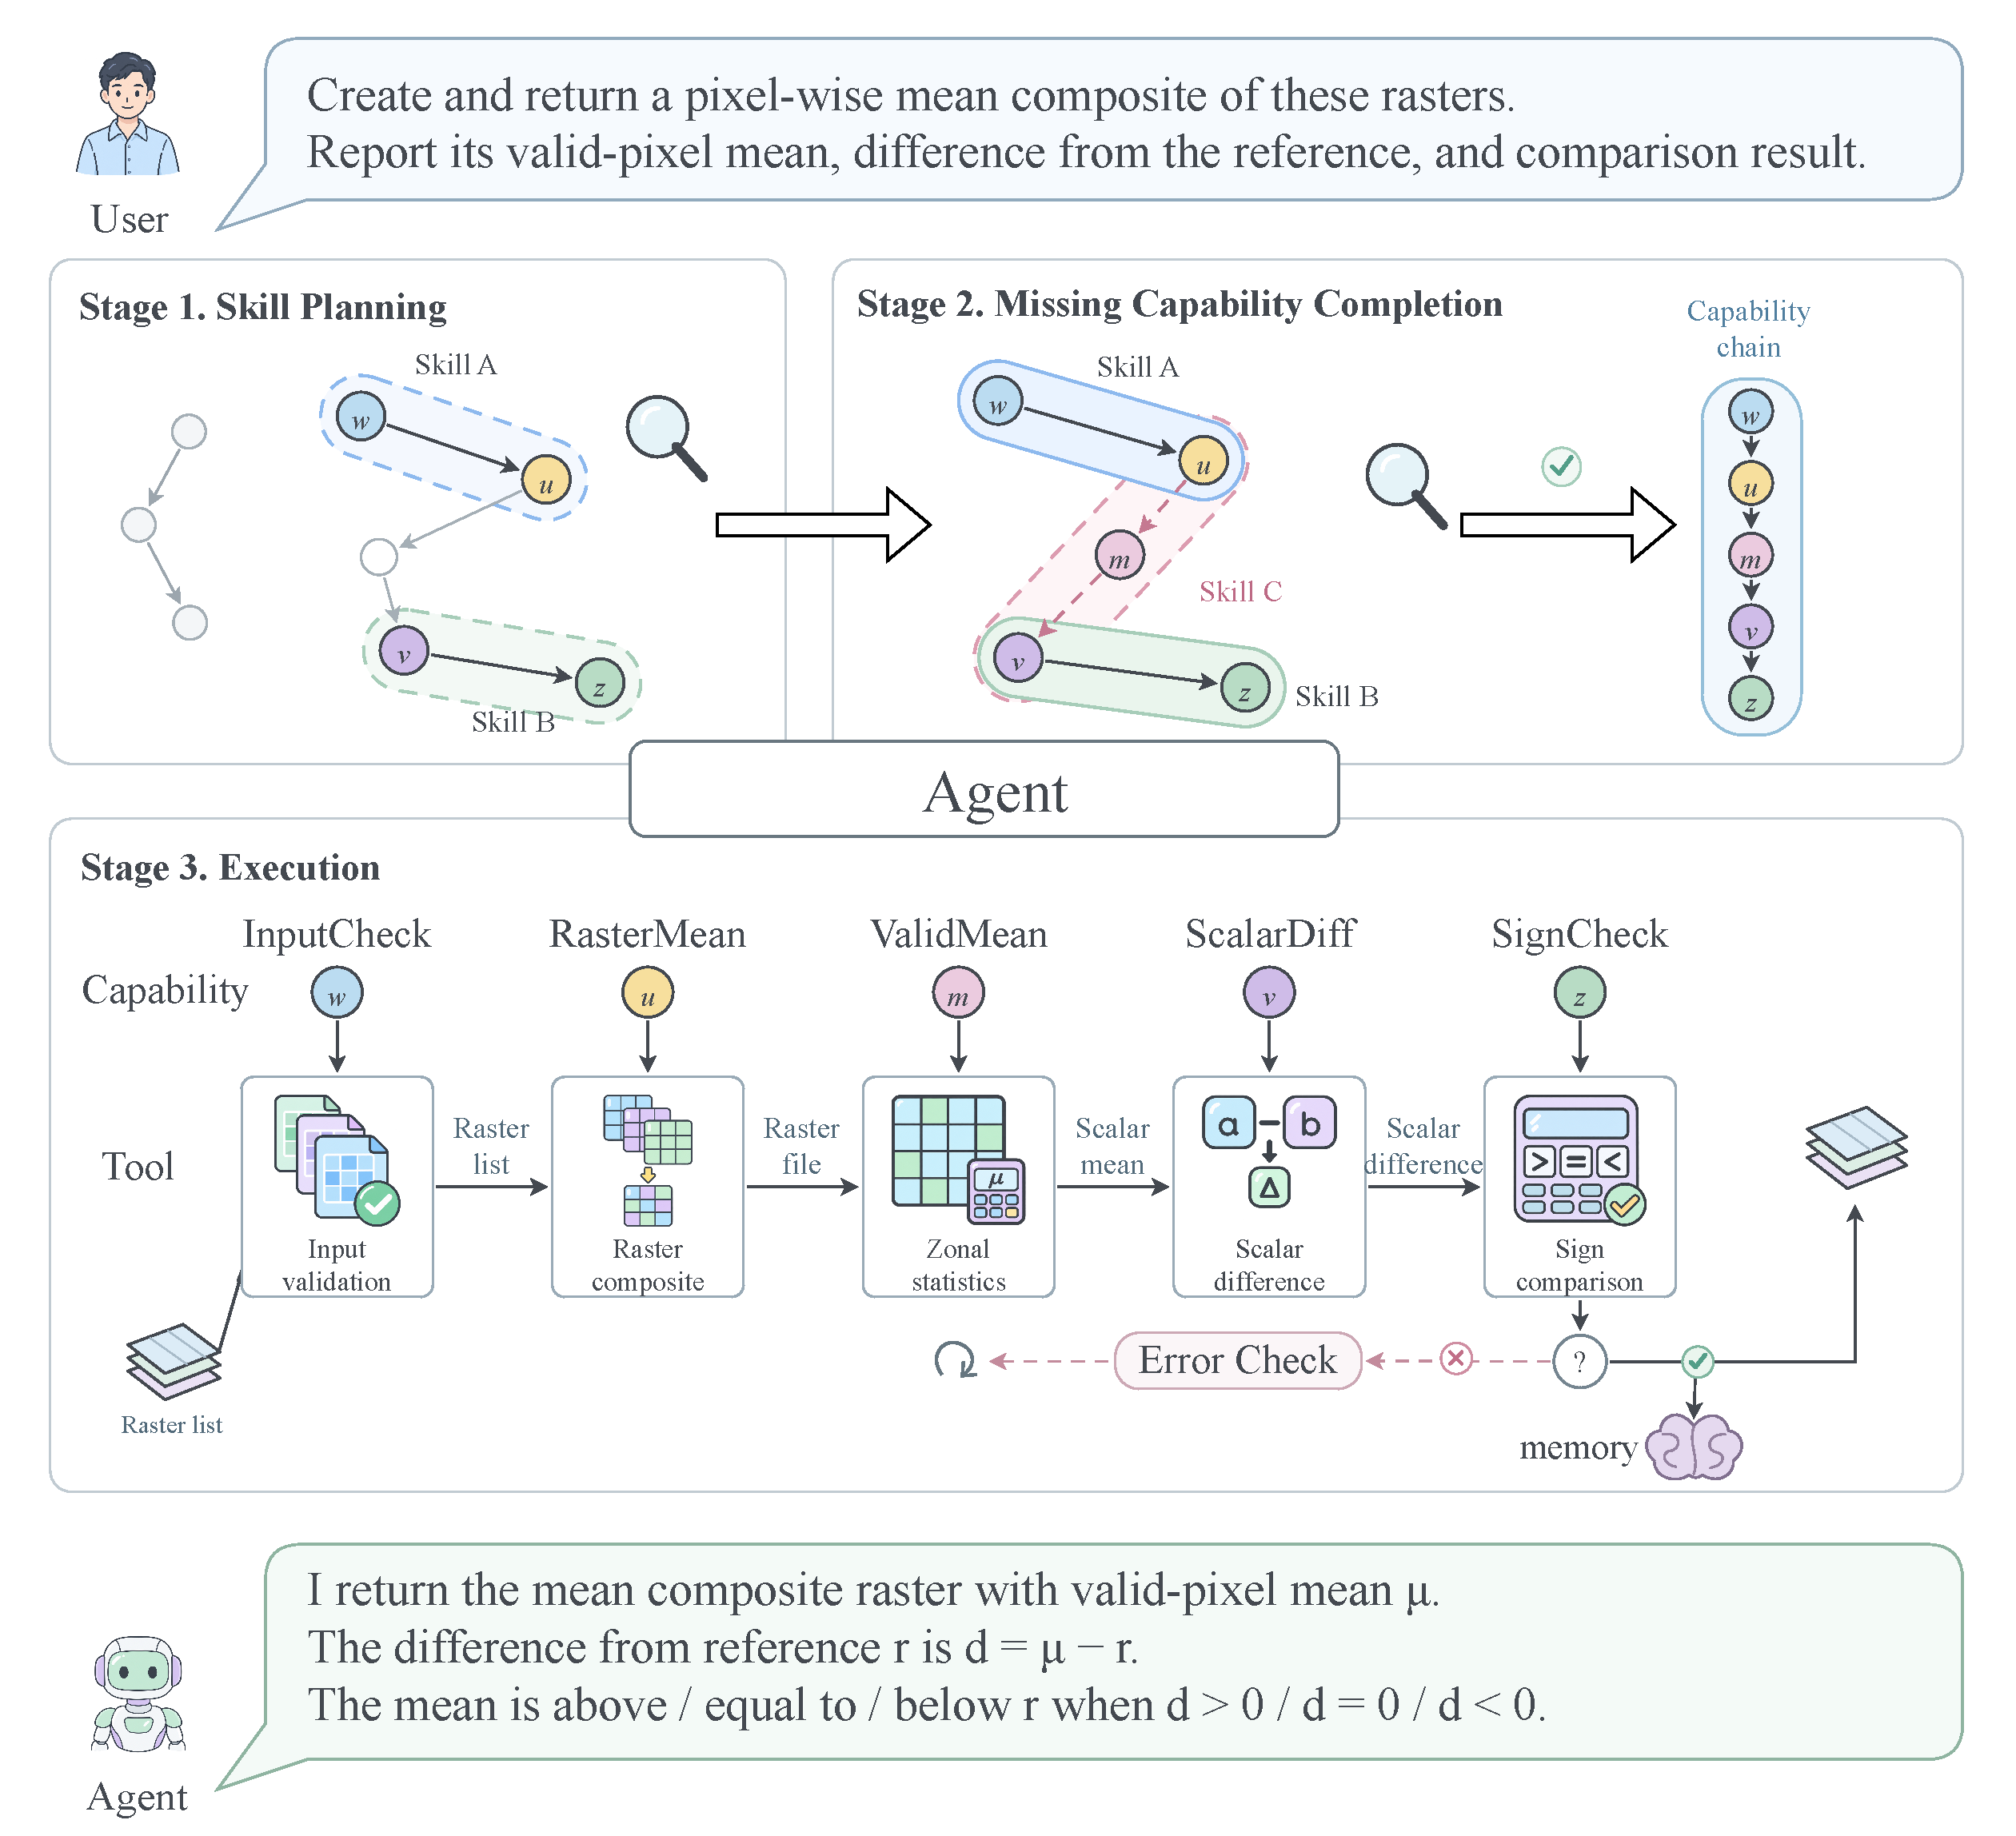
\includegraphics[width=0.83\textwidth]{case_study.pdf}
  \caption{Cross-Skill capability composition and tool execution. Stage 1 selects $w\to u$ from Skill $A$ and $v\to z$ from Skill $B$. Stage 2 inserts valid-pixel mean statistics $m$ using Skill $C$'s $u\to m\to v$ branch. Stage 3 grounds the five-step workflow in tool calls, propagates intermediate artifacts, and returns the composite raster, mean, difference, and comparison relation. The workflow is a mechanism illustration.}
  \label{fig:case-study}
  \Description{The case proceeds from two selected Skill fragments to a completed five-capability chain and corresponding input-validation, raster-compositing, zonal-statistics, scalar-differencing, and sign-comparison tools.}
\end{figure*}
